\documentclass[11pt,a4paper]{article}

\usepackage[T1]{fontenc}
\usepackage[utf8]{inputenc}
\usepackage{lmodern}
\usepackage{microtype}
\usepackage[a4paper,margin=22mm,headheight=22pt,headsep=10pt,footskip=11mm]{geometry}
\usepackage{xcolor}
\usepackage{graphicx}
\usepackage{tikz}
\usetikzlibrary{arrows.meta,automata,positioning,calc,fit,backgrounds}
\usepackage{booktabs}
\usepackage{tabularx}
\usepackage{longtable}
\usepackage{array}
\usepackage{enumitem}
\usepackage{listings}
\usepackage{fancyhdr}
\usepackage{titlesec}
\usepackage{tocloft}
\usepackage{adjustbox}
\usepackage{float}
\usepackage{needspace}
\usepackage{ragged2e}
\usepackage{xurl}
\usepackage[colorlinks=true,linkcolor=pupmaroon,urlcolor=pupmaroon,citecolor=pupmaroon]{hyperref}

\definecolor{pupmaroon}{HTML}{800000}
\definecolor{pupdark}{HTML}{4A1010}
\definecolor{pupgold}{HTML}{D9A928}
\definecolor{pupcream}{HTML}{FBF7EE}
\definecolor{ink}{HTML}{222222}
\definecolor{codebg}{HTML}{F6F1E7}
\definecolor{codeframe}{HTML}{D5C6AA}
\definecolor{commentgreen}{HTML}{3D6D4F}
\definecolor{stringblue}{HTML}{245B78}

\hypersetup{
  pdftitle={LAlgo: A Domain-Specific Programming Language Specification},
  pdfsubject={Language design specification for data structures and algorithms},
  pdfcreator={LaTeX}
}

\setlength{\parindent}{0pt}
\setlength{\parskip}{5.5pt plus 1pt minus 1pt}
\emergencystretch=3em
\clubpenalty=10000
\widowpenalty=10000
\displaywidowpenalty=10000
\setlist{leftmargin=1.55em,itemsep=2.5pt,topsep=4pt}

\titleformat{\section}{\Large\bfseries\color{pupmaroon}}{\thesection}{0.7em}{}
\titleformat{\subsection}{\large\bfseries\color{pupdark}}{\thesubsection}{0.65em}{}
\titleformat{\subsubsection}{\normalsize\bfseries\color{pupmaroon}}{\thesubsubsection}{0.6em}{}
\titlespacing*{\section}{0pt}{16pt}{7pt}
\titlespacing*{\subsection}{0pt}{12pt}{5pt}
\titlespacing*{\subsubsection}{0pt}{10pt}{4pt}

\renewcommand{\cftsecfont}{\bfseries\color{pupdark}}
\renewcommand{\cftsecpagefont}{\bfseries\color{pupdark}}
\renewcommand{\cftsubsecfont}{\color{ink}}
\renewcommand{\cftsubsecpagefont}{\color{ink}}
\setlength{\cftbeforesecskip}{4pt}

\pagestyle{fancy}
\fancyhf{}
\fancyhead[L]{\small\bfseries\color{pupmaroon}LAlgo - Language Design Specification}
\fancyhead[R]{\small\color{gray}BSCS 3-1 \textbar{} Group 4}
\fancyfoot[R]{\small\bfseries\color{pupmaroon}\thepage}
\renewcommand{\headrulewidth}{0.4pt}
\renewcommand{\headrule}{\vskip-8pt\hbox to\headwidth{\color{pupmaroon}\leaders\hrule height\headrulewidth\hfill}\vskip8pt}

\newcolumntype{Y}{>{\RaggedRight\arraybackslash}X}
\newcolumntype{L}[1]{>{\RaggedRight\arraybackslash}p{#1}}
\newcommand{\kw}[1]{\texttt{\bfseries\color{pupmaroon}#1}}
\newcommand{\token}[1]{\texttt{#1}}
\newcommand{\codeinline}[1]{\texttt{#1}}
\newcommand{\sectionrule}{}
\newcommand{\note}[1]{%
  \begin{center}\begin{minipage}{0.94\linewidth}
  \colorbox{pupcream}{\parbox{\dimexpr\linewidth-2\fboxsep\relax}{\small\textbf{Note.} #1}}
  \end{minipage}\end{center}}

\lstdefinelanguage{LAlgo}{
  morekeywords={INTEGER,DECIMAL,CHARACTER,BOOLEAN,ARRAY,STRING,IF,ELSE,WHILE,FOR,INPUT,OUTPUT,ALGORITHM,RETURN,TRACE,INVARIANT,TRUE,FALSE,DIV,AND,OR,NOT,SET,THE},
  sensitive=true,
  morecomment=[l]{//},
  morecomment=[s]{/*}{*/},
  morestring=[b]",
  morestring=[b]'
}
\lstset{
  language=LAlgo,
  basicstyle=\small\ttfamily,
  keywordstyle=\bfseries\color{pupmaroon},
  commentstyle=\itshape\color{commentgreen},
  stringstyle=\color{stringblue},
  backgroundcolor=\color{codebg},
  frame=single,
  rulecolor=\color{codeframe},
  framesep=6pt,
  xleftmargin=7pt,
  xrightmargin=7pt,
  aboveskip=7pt,
  belowskip=7pt,
  showstringspaces=false,
  columns=fullflexible,
  keepspaces=true,
  breaklines=true,
  breakatwhitespace=false,
  upquote=true
}

\tikzset{
  >={Stealth[length=2.2mm]},
  every state/.style={draw=pupmaroon,thick,fill=white,minimum size=9mm,font=\small},
  accepting/.style={double distance=1.5pt},
  start/.style={initial,initial text={start}},
  edge label/.style={fill=white,inner sep=1.5pt,font=\scriptsize,text=ink,align=center},
  every loop/.style={looseness=6}
}

\begin{document}

\hypersetup{pageanchor=false}
\begin{titlepage}
\thispagestyle{empty}
\vspace*{4mm}
\begin{center}
  
\includegraphics[width=32mm]{img/PUPLogo.png}\par
  \vspace{5mm}
  {\large Republic of the Philippines\par}
  \vspace{2mm}
  {\Large\bfseries POLYTECHNIC UNIVERSITY OF THE PHILIPPINES\par}
  \vspace{2mm}
  {\large College of Computer and Information Sciences\par}
  {\large Sta. Mesa, Manila\par}
  \vspace{7mm}
  {\fontsize{34}{40}\selectfont\bfseries\color{pupmaroon}LAlgo\par}
  \vspace{3mm}
  {\LARGE\bfseries\color{pupmaroon}Language Design Specification\par}
  \vspace{5mm}
  {\large A Domain-Specific Language for Observable Execution,\par
  Tracing, and Reasoning in Algorithms\par}
  \vspace{3mm}
  {\large\itshape Formal Syntax and Operational Lexicon\par}
  \vspace{6mm}
  {\large\bfseries Submitted by: Group 4\par}
  \vspace{3mm}
  {\large
  Buenaventura, Harvey L.\par
  De Mesa, Joshua C.\par
  Dela Rosa, Mico Von Adriel A.\par
  Magalona, Adriel M.\par
  Morales, Timothy Gabriel\par
  Nevado, Sean Andrew M.\par
  Salvacion, Dean James G.\par}
  \vspace{4mm}
  {\large\bfseries Submitted to\par}
  \vspace{2mm}
  {\large Prof. Ria A. Sagum\par}
  \vspace{3mm}
  {\large\bfseries Course and Subject Code\par}
  \vspace{2mm}
  {\large Principles of Programming Languages (COSC 303)\par}
\end{center}
\end{titlepage}

\hypersetup{pageanchor=true}
\pagenumbering{roman}
\begingroup
\small
\tableofcontents
\endgroup
\clearpage
\pagenumbering{arabic}

\section{Introduction}
\sectionrule

\subsection{Overview}

LAlgo is a proposed imperative domain-specific language (DSL) for expressing data structures and algorithms (DSA) in readable pseudocode. This proposal focuses on the lexical analyzer: the character alphabet, token classes, and one unified deterministic finite automaton used to recognize source text. A complete parser and runtime are future work.

The examples use familiar declarations, operators, indexing, and control-flow words to show the intended token vocabulary. They illustrate how an algorithm such as binary search could be written, but they do not claim that execution tracing or invariant checking is implemented by the present lexical proposal.

\subsection{Inspiration}

The primary inspiration for LAlgo emerges from the cognitive disconnect students encounter when transitioning between algorithmic pseudocode and practical code implementation. Textbooks routinely present algorithms alongside step-by-step state trace tables and formal loop assertions. However, translating these designs into standard programming environments forces students to manage language-specific boilerplate, unmonitored variable states, and implicit type conversions that mask algorithmic errors.

When a learner encounters an off-by-one error, the sequence of intermediate states can be difficult to reconstruct. LAlgo draws inspiration from educational pseudocode, Pascal-like syntax, and structured tracing tools. This paper establishes the lexical groundwork for that longer-term direction without specifying a tracing runtime.

\subsection{Problem Addressed}

Traditional programming language compilers and runtime engines are intentionally opaque: they consume source code, optimize away intermediate variables, and produce final output. Under this execution model:

\begin{center}
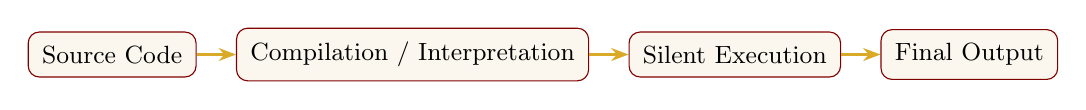
\begin{tikzpicture}[node distance=8mm and 5mm,font=\small]
  \node[draw=pupmaroon,rounded corners,fill=pupcream,inner sep=5pt] (src) {Source Code};
  \node[draw=pupmaroon,rounded corners,fill=pupcream,inner sep=5pt,right=of src] (comp) {Compilation / Interpretation};
  \node[draw=pupmaroon,rounded corners,fill=pupcream,inner sep=5pt,right=of comp] (silent) {Silent Execution};
  \node[draw=pupmaroon,rounded corners,fill=pupcream,inner sep=5pt,right=of silent] (out) {Final Output};
  \draw[->,thick,pupgold] (src)--(comp);
  \draw[->,thick,pupgold] (comp)--(silent);
  \draw[->,thick,pupgold] (silent)--(out);
\end{tikzpicture}
\end{center}

This pipeline introduces several core educational problems:

\begin{itemize}
  \item \textbf{Silent Intermediate States.} Students observe only terminal outputs, leaving internal invariant breakdowns, element swaps, and path traversals invisible.
  \item \textbf{Unverified Invariants.} Algorithmic correctness proofs rely on inductive loop invariants, yet standard languages provide no native, readable syntactic construct to express whether loop conditions remain valid across iterations.
  \item \textbf{Hidden State Changes.} Intermediate variable updates and branch decisions can be difficult to follow without manually adding diagnostic output.
\end{itemize}

The present proposal addresses the lexical foundation of this problem. Parsing, execution-state observation, and any later tracing or verification behavior require separate specifications.

\Needspace{12\baselineskip}
\subsection{Objectives}

The primary goal of this iteration is to define an unambiguous token vocabulary and deterministic lexical recognition model for algorithmic source text. Specifically, the project aims to:

\begin{enumerate}
  \item Define an unambiguous lexical structure and formal automata suited for algorithmic problem solving.
  \item Recognize tokens used by illustrative declarations, I/O, assignments, conditional branches, and loops without defining their full parser or runtime behavior.
  \item Recognize collection-type words (\kw{ARRAY} and \kw{STRING}) and the associated delimiters.
  \item Reserve \kw{ALGORITHM}, \kw{RETURN}, \kw{TRACE}, and \kw{INVARIANT} for possible future syntactic extensions, without assigning them executable behavior in this iteration.
\end{enumerate}

\section{Lexical Elements}
\sectionrule

\subsection{Character Set}

LAlgo utilizes a standard ASCII-based character set denoted by the finite alphabet $\Sigma$. The alphabet is organized into lexical classes:

\[
\begin{array}{@{}l}
\Sigma = \Sigma_{\mathrm{alpha}} \cup \Sigma_{\mathrm{digits}} \cup
\Sigma_{\mathrm{arithmetic}} \cup \Sigma_{\mathrm{relational}} \cup
\Sigma_{\mathrm{delimiters}}\\
\hspace{1.2cm}{} \cup \Sigma_{\mathrm{underscore}} \cup
\Sigma_{\mathrm{quotes}} \cup \Sigma_{\mathrm{whitespace}} \cup
\Sigma_{\mathrm{literal}} \cup \Sigma_{\mathrm{comment}}.
\end{array}
\]

The supported character categories are explicitly defined below.

\begin{description}[leftmargin=0pt,labelindent=0pt,labelwidth=0pt,itemindent=0pt]
  \item[Alphabetic Characters ($\Sigma_{\mathrm{alpha}}$)]
  \codeinline{a b c d e f g h i j k l m n o p q r s t u v w x y z}\newline
  \codeinline{A B C D E F G H I J K L M N O P Q R S T U V W X Y Z}
  \item[Numeric Digits ($\Sigma_{\mathrm{digits}}$)]
  \codeinline{0 1 2 3 4 5 6 7 8 9}
  \item[Arithmetic Symbols ($\Sigma_{\mathrm{arithmetic}}$)]
  \codeinline{+ - * / \% \textasciicircum}
  \item[Relational and Assignment Symbols ($\Sigma_{\mathrm{relational}}$)]
  \codeinline{= ! < >}
  \item[Delimiters and Punctuation ($\Sigma_{\mathrm{delimiters}}$)]
  \codeinline{( ) [ ] \{ \} , ; : .}
  \item[Identifier Continuation Symbol ($\Sigma_{\mathrm{underscore}}$)]
  \codeinline{\_}
  \item[Quotation Symbols ($\Sigma_{\mathrm{quotes}}$)]
  \codeinline{" '}
  \item[Whitespace Characters ($\Sigma_{\mathrm{whitespace}}$)]
  Space (ASCII 32), horizontal tab (ASCII 9), and line feed (ASCII 10).
  \item[Literal/Comment-Only Symbols ($\Sigma_{\mathrm{literal}}$)]
  Printable ASCII 33--126 not already in another class and other than backslash; these symbols are permitted only inside quoted literals and comments.
  \item[Comment-Only Symbol ($\Sigma_{\mathrm{comment}}$)]
  Backslash (ASCII 92), permitted in comments only; it does not introduce an escape.
\end{description}

Space and horizontal tab are also permitted inside string literals, character literals, and comments, even though they belong to $\Sigma_{\mathrm{whitespace}}$.

The scanner combines the individual relational characters into \codeinline{==}, \codeinline{!=}, \codeinline{<=}, and \codeinline{>=} using lookahead. These are multi-character operators rather than additional members of the character alphabet; \codeinline{!} alone is not a valid operator.

\subsection{Identifiers}

Identifiers are programmer-defined tokens used to name variables, constants, and algorithmic routines. An identifier must satisfy the following lexical constraints:

\begin{itemize}
  \item It must begin with an alphabetic character (\codeinline{a-z} or \codeinline{A-Z}).
  \item It may subsequently contain alphabetic characters, numeric digits (\codeinline{0-9}), or underscores (\codeinline{\_}).
  \item It must not match any reserved keyword or noise word.
  \item It is strictly case-sensitive: \codeinline{counter}, \codeinline{Counter}, and \codeinline{COUNTER} are distinct tokens.
\end{itemize}

Formally, the lexical structure of an identifier is expressed by the regular expression:

\begin{lstlisting}[language={},basicstyle=\normalsize\ttfamily]
[a-zA-Z][a-zA-Z0-9_]*
\end{lstlisting}

\begin{minipage}[t]{0.47\linewidth}
\textbf{Valid identifiers}
\begin{lstlisting}[language={}]
low
high
binarySearch
target_index
arraySize2
\end{lstlisting}
\end{minipage}\hfill
\begin{minipage}[t]{0.50\linewidth}
\textbf{Invalid identifiers}
\begin{lstlisting}[language={},breaklines=true]
2low // Lexical error: number followed by letter
target-index // Hyphen means subtraction
WHILE        // Reserved keyword
SET          // Reserved noise word
\end{lstlisting}
\end{minipage}

\subsection{Finite Automata (Lexical Analyzer Execution Model)}

LAlgo's implemented lexical scanner processes raw source code using one unified deterministic finite automaton (DFA), with one start state and one shared transition table. Formally, the automaton is defined as a five-tuple:

\[
M = (Q, \Sigma, \delta, q_0, F),
\]

where $Q$ is the finite set of internal states, $\Sigma$ is the input character alphabet, $\delta:Q\times\Sigma\to Q$ is the state transition function, $q_0\in Q$ is the initial state, and $F\subseteq Q$ is the set of accepting states.

Diagrams show only defined transitions; every missing transition goes to an implicit non-accepting error state, so $\delta$ is total. State sets listed below omit this implicit state for readability. The scanner remembers the last accepting position and leaves lookahead for the next token. Entering the error state ends a candidate match; it reports an error only if no valid token can be emitted or an explicit lexical restriction is violated. Once a quote or comment opener is recognized, an unterminated construct is an error, not a fallback to a shorter token.

\Needspace{30\baselineskip}
\subsubsection{Unified DFA with One Start State}\label{sec:unified}

The implementation in \codeinline{lalgo\_unified.c} builds one table, \codeinline{DELTA[state][class]}, with 254 explicit states and 83 input classes. Every candidate lexeme starts at the same $q_0$. Keywords, identifiers, numeric literals, operators, comments, quoted literals, delimiters, and whitespace are paths within this single state graph. There is no runtime dispatch to separate recognizers and no post-scan string comparison for keywords.

The figure below is a grouped overview of the unified graph, not a substitute for its complete transitions. Each box denotes a state family; keyword letters and individual punctuation have distinct concrete states. Appendix~\ref{app:unified} gives every state, accepting action, and defined transition directly from the C implementation. The category diagrams that follow use local state labels as explanatory projections of these paths; they are not independently executed DFAs and their local $q_0$ denotes the same global start.

After each transition the scanner remembers the last accepting state and source position. It emits the longest accepted prefix, retains unused lookahead, then restarts at $q_0$ for the next lexeme. Whitespace accepts with a skip action. A malformed-number state accepts an INVALID candidate for diagnostic reporting. Unterminated quoted literals and block comments use committed-state metadata to prevent fallback to a shorter token. These scanner actions are distinct from DFA transitions.

\begin{figure}[H]
\centering
\begin{adjustbox}{max width=\linewidth}
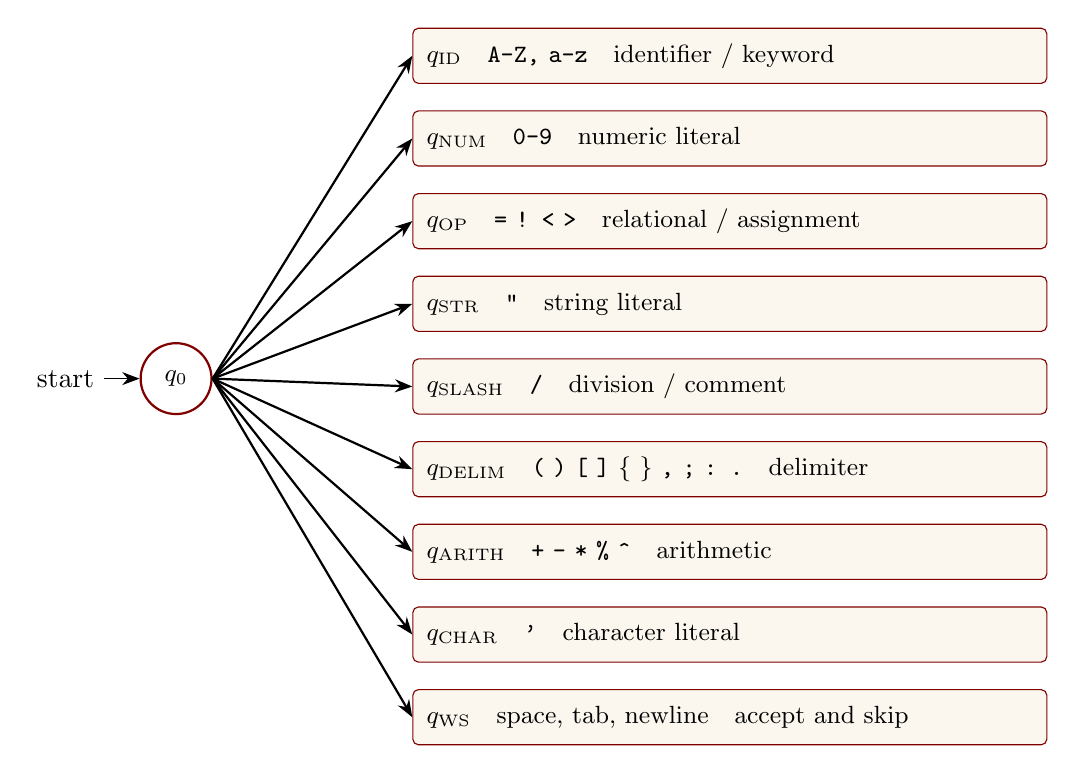
\begin{tikzpicture}[
  route/.style={draw=pupmaroon,rounded corners=2pt,fill=pupcream,
    text width=7.7cm,minimum height=7mm,align=left,font=\small,inner xsep=5pt}
]
  \node[state,start] (q0) at (0,0) {$q_0$};
  \node[route,anchor=west] (qid) at (3,4.1) {$q_{\mathrm{ID}}$\quad \texttt{A-Z, a-z}\quad identifier / keyword};
  \node[route,anchor=west] (qnum) at (3,3.05) {$q_{\mathrm{NUM}}$\quad \texttt{0-9}\quad numeric literal};
  \node[route,anchor=west] (qop) at (3,2.0) {$q_{\mathrm{OP}}$\quad \texttt{= ! < >}\quad relational / assignment};
  \node[route,anchor=west] (qstr) at (3,0.95) {$q_{\mathrm{STR}}$\quad \texttt{"}\quad string literal};
  \node[route,anchor=west] (qslash) at (3,-0.1) {$q_{\mathrm{SLASH}}$\quad \texttt{/}\quad division / comment};
  \node[route,anchor=west] (qdelim) at (3,-1.15) {$q_{\mathrm{DELIM}}$\quad \texttt{( ) [ ] \{ \} , ; : .}\quad delimiter};
  \node[route,anchor=west] (qarith) at (3,-2.2) {$q_{\mathrm{ARITH}}$\quad \texttt{+ - * \% \textasciicircum}\quad arithmetic};
  \node[route,anchor=west] (qchar) at (3,-3.25) {$q_{\mathrm{CHAR}}$\quad \texttt{'}\quad character literal};
  \node[route,anchor=west] (qws) at (3,-4.3) {$q_{\mathrm{WS}}$\quad space, tab, newline\quad accept and skip};
  \draw[->,thick] (q0.east) -- (qws.west);
  \draw[->,thick] (q0.east) -- (qid.west);
  \draw[->,thick] (q0.east) -- (qnum.west);
  \draw[->,thick] (q0.east) -- (qop.west);
  \draw[->,thick] (q0.east) -- (qstr.west);
  \draw[->,thick] (q0.east) -- (qslash.west);
  \draw[->,thick] (q0.east) -- (qdelim.west);
  \draw[->,thick] (q0.east) -- (qarith.west);
  \draw[->,thick] (q0.east) -- (qchar.west);

\end{tikzpicture}
\end{adjustbox}
\caption{Grouped overview of one unified DFA: all token families branch from the single start state $q_0$.}
\end{figure}

\Needspace{24\baselineskip}
\textbf{Step-by-step lexical scan trace.} Consider the statement \codeinline{count = 10}.

\begin{table}[H]
\centering\small
\begin{tabularx}{\linewidth}{>{\bfseries}c L{17mm} L{28mm} Y Y}
\toprule
Step & Current state & Character(s) & Automaton action & Token emitted \\
\midrule
1 & $q_0$ & \codeinline{'c'} & Transition to $q_{\mathrm{ID}}$ & None \\
2 & $q_{\mathrm{ID}}$ & \codeinline{'o', 'u',}\newline\codeinline{'n', 't'} & Self-loop on $q_{\mathrm{ID}}$ & None \\
3 & $q_{\mathrm{ID}}$ & space & No accepting extension; emit and reset & \token{TOKEN(IDENT,}\newline\token{"count")} \\
4 & $q_0$ & space & Consume whitespace recognizer & None \\
5 & $q_0$ & \codeinline{'='} & Transition to $q_{\mathrm{OP}}$ & None \\
6 & $q_{\mathrm{OP}}$ & space & Lookahead is not \codeinline{'='}; emit and reset & \token{TOKEN(ASSIGN,}\newline\token{"=")} \\
7 & $q_0$ & space & Consume whitespace recognizer & None \\
8 & $q_0$ & \codeinline{'1'} & Transition to $q_{\mathrm{NUM}}$ & None \\
9 & $q_{\mathrm{NUM}}$ & \codeinline{'0'} & Self-loop on $q_{\mathrm{NUM}}$ & None \\
10 & $q_{\mathrm{NUM}}$ & EOF & Buffer end; emit and reset & \token{TOKEN(INTEGER,}\newline\token{10)} \\
\bottomrule
\end{tabularx}
\end{table}

\Needspace{16\baselineskip}
\subsubsection{DFA for Identifiers and Keywords}

Identifiers begin with an alphabetic character and may continue with letters, digits, or underscores. This diagram projects the general identifier shape. In the full unified DFA, uppercase keyword-prefix states accept their associated token at complete spellings; a non-keyword continuation falls into the general identifier state. Lowercase or mixed-case prefix states accept IDENT and flag a complete keyword spelling as suspected. Keyword recognition is part of the same scan, not a later lookup.

\begin{itemize}
  \item $Q=\{q_0,q_1\}$
  \item $q_0$: initial state
  \item $F=\{q_1\}$ (accepting state)
\end{itemize}

\begin{center}
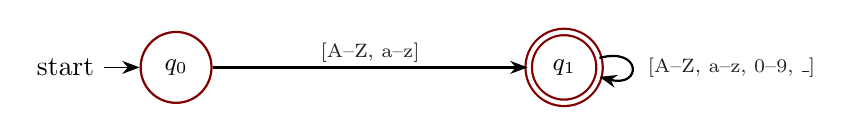
\begin{tikzpicture}[node distance=40mm]
  \node[state,start] (q0) {$q_0$};
  \node[state,accepting,right=of q0] (q1) {$q_1$};
  \path[->,thick]
    (q0) edge node[edge label,above] {[A--Z, a--z]} (q1)
    (q1) edge[loop right] node[edge label,right=4pt] {[A--Z, a--z, 0--9, \_]} (q1);
\end{tikzpicture}
\end{center}

\subsubsection{DFA for Numeric Literals (Integer and Decimal)}

This automaton distinguishes whole-number values (\kw{INTEGER}) from fractional real numbers (\kw{DECIMAL}) through decimal-point transitions.

\begin{itemize}
  \item $Q=\{q_0,q_1,q_2,q_3\}$
  \item $F=\{q_1,q_3\}$, where $q_1$ accepts \kw{INTEGER} and $q_3$ accepts \kw{DECIMAL}
\end{itemize}

\begin{center}
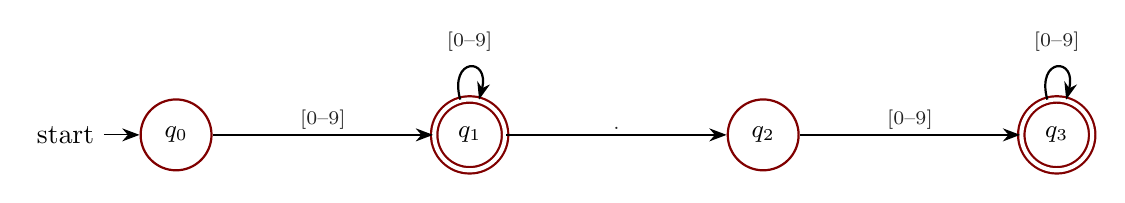
\begin{tikzpicture}[node distance=28mm]
  \node[state,start] (q0) {$q_0$};
  \node[state,accepting,right=of q0] (q1) {$q_1$};
  \node[state,right=of q1] (q2) {$q_2$};
  \node[state,accepting,right=of q2] (q3) {$q_3$};
  \path[->,thick]
    (q0) edge node[edge label,above] {[0--9]} (q1)
    (q1) edge[loop above] node[edge label,above=4pt] {[0--9]} (q1)
    (q1) edge node[edge label,above] {.} (q2)
    (q2) edge node[edge label,above] {[0--9]} (q3)
    (q3) edge[loop above] node[edge label,above=4pt] {[0--9]} (q3);
\end{tikzpicture}
\end{center}

\begin{itemize}
  \item \textbf{Trailing dot.} \codeinline{3.} is not a \token{DECIMAL}. From non-accepting $q_2$, the scanner backtracks to the last accepting position and emits \token{INTEGER} \codeinline{3}, followed by \token{DOT}.
  \item \textbf{Leading dot.} \codeinline{.5} is \token{DOT} followed by \token{INTEGER} \codeinline{5}. A decimal requires at least one digit on each side of the point.
  \item \textbf{Leading zeros.} Allowed and ignored in value: \codeinline{007} = 7 and \codeinline{00.5} = 0.5. The original spelling remains in the token's lexeme.
  \item \textbf{Range.} Integer literals must fit the signed 32-bit range; their maximum unsigned magnitude is 2147483647. Larger literals are lexical errors. Since signs are separate operators, even the magnitude 2147483648 in \codeinline{-2147483648} is rejected. Double precision is the proposed runtime representation for decimals; this lexer recognizes decimal spelling without converting values or checking floating-point range.
\end{itemize}

\Needspace{22\baselineskip}
\subsubsection{DFA for Relational and Assignment Operators}

This DFA disambiguates single-character assignment and comparison operators (\codeinline{=}, \codeinline{<}, \codeinline{>}) from compound relational operators (\codeinline{==}, \codeinline{!=}, \codeinline{<=}, \codeinline{>=}).

\begin{itemize}
  \item $Q=\{q_0,q_1,q_2,q_3,q_4,q_5,q_6\}$
  \item $F=\{q_1,q_2,q_4,q_5,q_6\}$
\end{itemize}

\begin{center}
\begin{adjustbox}{max width=\linewidth}
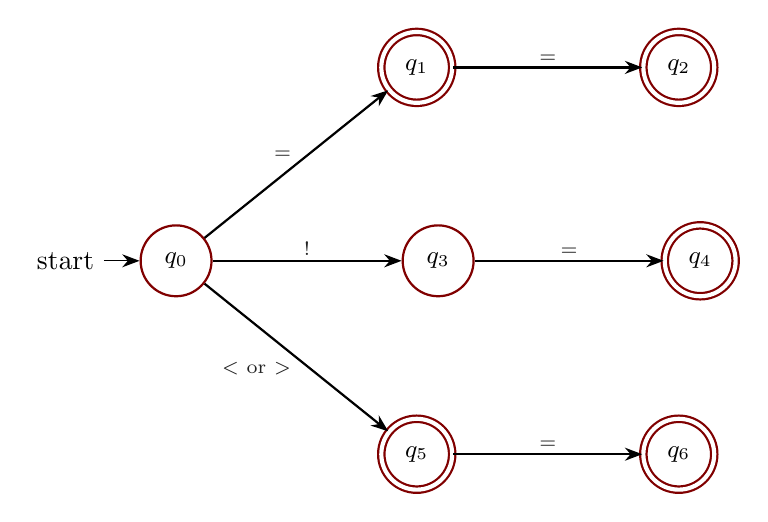
\begin{tikzpicture}[node distance=18mm and 24mm]
  \node[state,start] (q0) {$q_0$};
  \node[state,accepting,above right=of q0] (q1) {$q_1$};
  \node[state,accepting,right=of q1] (q2) {$q_2$};
  \node[state,right=of q0] (q3) {$q_3$};
  \node[state,accepting,right=of q3] (q4) {$q_4$};
  \node[state,accepting,below right=of q0] (q5) {$q_5$};
  \node[state,accepting,right=of q5] (q6) {$q_6$};
  \path[->,thick]
    (q0) edge node[edge label,above left] {=} (q1)
    (q1) edge node[edge label,above] {=} (q2)
    (q0) edge node[edge label,above] {!} (q3)
    (q3) edge node[edge label,above] {=} (q4)
    (q0) edge node[edge label,below left] {$<$ or $>$} (q5)
    (q5) edge node[edge label,above] {=} (q6);
\end{tikzpicture}
\end{adjustbox}
\end{center}

\Needspace{25\baselineskip}
\subsubsection{DFA for Comments and Division}

Transition labels such as ``other'' and ``non-*'' range only over the permitted comment-body characters in Section~\ref{sec:comments}; unsupported characters are lexical errors.

This DFA distinguishes division (\codeinline{/}) from single-line comments (\codeinline{//}) and block comments (\codeinline{/* ... */}) using lookahead scanning.

\begin{itemize}
  \item $Q=\{q_0,q_1,q_2,q_3,q_4,q_5\}$
  \item $F=\{q_1,q_2,q_5\}$, where $q_1$ accepts division, $q_2$ accepts a single-line comment, and $q_5$ accepts a multi-line comment
\end{itemize}

\begin{center}
\begin{adjustbox}{max width=\linewidth}
\begin{tikzpicture}[node distance=18mm and 24mm]
  \node[state,start] (q0) {$q_0$};
  \node[state,accepting,right=of q0] (q1) {$q_1$};
  \node[state,accepting,above right=of q1] (q2) {$q_2$};
  \node[state,below right=of q1] (q3) {$q_3$};
  \node[state,right=of q3] (q4) {$q_4$};
  \node[state,accepting,right=of q4] (q5) {$q_5$};
  \path[->,thick]
    (q0) edge node[edge label,above] {/} (q1)
    (q1) edge node[edge label,above left] {/} (q2)
    (q2) edge[loop above] node[edge label,above=4pt] {any except newline} (q2)
    (q1) edge node[edge label,below left] {*} (q3)
    (q3) edge[loop below] node[edge label,below=4pt] {non-*} (q3)
    (q3) edge[bend left=14] node[edge label,above] {*} (q4)
    (q4) edge[bend left=14] node[edge label,below] {other} (q3)
    (q4) edge[loop above] node[edge label,above=4pt] {*} (q4)
    (q4) edge node[edge label,above] {/} (q5);
\end{tikzpicture}
\end{adjustbox}
\end{center}

\Needspace{20\baselineskip}
\subsubsection{DFA for String Literals}

This DFA recognizes character-string literals enclosed by double quotation marks (\codeinline{"..."}). Their contents consist of printable ASCII characters other than a double quote or backslash, plus horizontal tab; escape sequences and embedded newlines are not defined.

\begin{itemize}
  \item $Q=\{q_0,q_1,q_2\}$
  \item $F=\{q_2\}$
\end{itemize}

\begin{center}
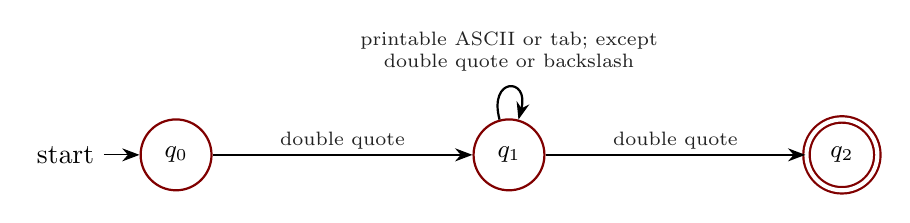
\begin{tikzpicture}[node distance=33mm]
  \node[state,start] (q0) {$q_0$};
  \node[state,right=of q0] (q1) {$q_1$};
  \node[state,accepting,right=of q1] (q2) {$q_2$};
  \path[->,thick]
    (q0) edge node[edge label,above] {double quote} (q1)
    (q1) edge[loop above] node[edge label,above=4pt,align=center] {printable ASCII or tab; except\\double quote or backslash} (q1)
    (q1) edge node[edge label,above] {double quote} (q2);
\end{tikzpicture}
\end{center}

\Needspace{13\baselineskip}
\subsubsection{DFA for Character Literals}\label{sec:character-dfa}

A character literal consists of one printable ASCII character or horizontal tab enclosed in single quotation marks, such as \codeinline{'A'} or \codeinline{','}. The character between the quotes may be ASCII 32--126 except a single quote or backslash, or a horizontal tab; escape sequences are not defined in this specification. An empty, multi-character, or unterminated literal is a lexical error.

\begin{itemize}
  \item $Q=\{q_0,q_1,q_2,q_3\}$
  \item $F=\{q_3\}$
\end{itemize}

\begin{center}
\begin{adjustbox}{max width=\linewidth}
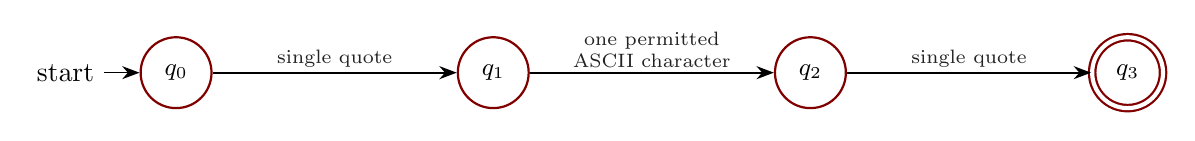
\begin{tikzpicture}[node distance=31mm]
  \node[state,start] (q0) {$q_0$};
  \node[state,right=of q0] (q1) {$q_1$};
  \node[state,right=of q1] (q2) {$q_2$};
  \node[state,accepting,right=of q2] (q3) {$q_3$};
  \path[->,thick]
    (q0) edge node[edge label,above] {single quote} (q1)
    (q1) edge node[edge label,above,align=center] {one permitted\\ASCII character} (q2)
    (q2) edge node[edge label,above] {single quote} (q3);
\end{tikzpicture}
\end{adjustbox}
\end{center}

\subsubsection{DFA for Whitespace (Blanks)}\label{sec:whitespace-dfa}

Whitespace characters---spaces, horizontal tabs, and line feeds---are recognized by a trivial single-loop automaton. Tokens matched by this automaton are consumed by the lexer but are not emitted to the parser; they separate adjacent lexemes and update source positions and newline metadata.

\begin{itemize}
  \item $Q=\{q_0,q_1\}$
  \item $F=\{q_1\}$ (accepting, but discarded)
\end{itemize}

\begin{center}
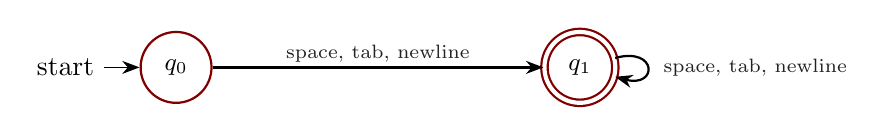
\begin{tikzpicture}[node distance=42mm]
  \node[state,start] (q0) {$q_0$};
  \node[state,accepting,right=of q0] (q1) {$q_1$};
  \path[->,thick]
    (q0) edge node[edge label,above] {space, tab, newline} (q1)
    (q1) edge[loop right] node[edge label,right=4pt] {space, tab, newline} (q1);
\end{tikzpicture}
\end{center}

Because whitespace carries no semantic weight (Section~\ref{sec:whitespace}), the scanner discards any accepted whitespace lexeme instead of forwarding it to the parser, preserves any line-feed information in token metadata, then resumes scanning from $q_0$.

\Needspace{13\baselineskip}
\subsubsection{DFA for Delimiters and Brackets}

Delimiters and brackets are single-character tokens: \codeinline{( ) [ ] \{ \} , ; : .}. Because no lookahead is required, each is accepted after exactly one transition from $q_0$.

\begin{itemize}
  \item $Q=\{q_0,q_1\}$
  \item $F=\{q_1\}$, where the specific delimiter determines the emitted token type (for example, \token{LPAREN}, \token{RBRACE}, or \token{COMMA})
\end{itemize}

\begin{center}
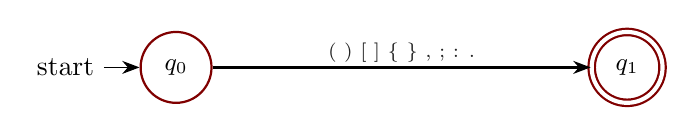
\begin{tikzpicture}[node distance=48mm]
  \node[state,start] (q0) {$q_0$};
  \node[state,accepting,right=of q0] (q1) {$q_1$};
  \path[->,thick] (q0) edge node[edge label,above] {( ) [ ] \{ \} , ; : .} (q1);
\end{tikzpicture}
\end{center}

Unlike the multi-character automata above, no maximal munch is needed: the lexer emits the corresponding token immediately after the single accepted transition and resets to $q_0$.

\Needspace{21\baselineskip}
\subsubsection{Representative DFA for Keyword Recognition}

The identifier DFA defines the shape shared by identifiers and reserved words: a letter followed by zero or more letters, digits, or underscores. The automaton below illustrates how that general shape narrows into the exact spelling of \kw{IF}, \kw{INPUT}, \kw{INTEGER}, and \kw{INVARIANT}. The first three are current language keywords; \kw{INVARIANT} is reserved for a future extension. They share the prefix \codeinline{I} and diverge as their spellings differ.

\begin{figure}[htbp]
\centering
\begin{adjustbox}{max width=\linewidth}
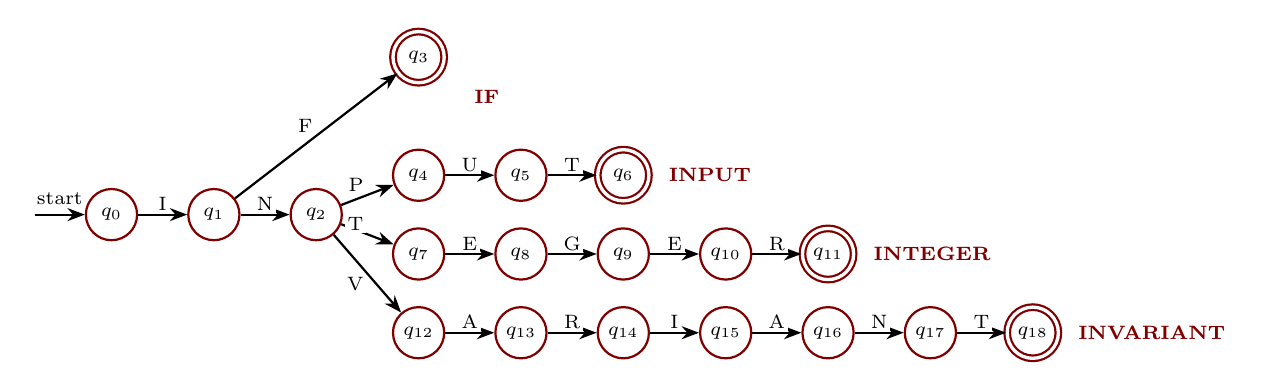
\begin{tikzpicture}[
  x=13mm,y=10mm,
  every node/.style={font=\scriptsize},
  key/.style={circle,draw=pupmaroon,thick,fill=white,minimum size=6.5mm,inner sep=0pt},
  acceptkey/.style={key,double,double distance=1.2pt},
  edge label/.style={fill=white,inner sep=1pt,font=\scriptsize}
]
  \node[key] (q0) at (0,0) {$q_0$};
  \node[key] (q1) at (1,0) {$q_1$};
  \node[key] (q2) at (2,0) {$q_2$};
  \node[acceptkey] (q3) at (3,2.0) {$q_3$};
  \node[key] (q4) at (3,0.5) {$q_4$};
  \node[key] (q5) at (4,0.5) {$q_5$};
  \node[acceptkey] (q6) at (5,0.5) {$q_6$};
  \node[key] (q7) at (3,-0.5) {$q_7$};
  \node[key] (q8) at (4,-0.5) {$q_8$};
  \node[key] (q9) at (5,-0.5) {$q_9$};
  \node[key] (q10) at (6,-0.5) {$q_{10}$};
  \node[acceptkey] (q11) at (7,-0.5) {$q_{11}$};
  \node[key] (q12) at (3,-1.5) {$q_{12}$};
  \node[key] (q13) at (4,-1.5) {$q_{13}$};
  \node[key] (q14) at (5,-1.5) {$q_{14}$};
  \node[key] (q15) at (6,-1.5) {$q_{15}$};
  \node[key] (q16) at (7,-1.5) {$q_{16}$};
  \node[key] (q17) at (8,-1.5) {$q_{17}$};
  \node[acceptkey] (q18) at (9,-1.5) {$q_{18}$};
  \draw[->,thick] (-0.75,0)--(q0) node[midway,above,font=\scriptsize]{start};
  \draw[->,thick] (q0)--node[edge label,above]{I}(q1);
  \draw[->,thick] (q1)--node[edge label,above]{N}(q2);
  \draw[->,thick] (q1)--node[edge label,above left]{F}(q3);
  \draw[->,thick] (q2)--node[edge label,above left]{P}(q4);
  \draw[->,thick] (q4)--node[edge label,above]{U}(q5);
  \draw[->,thick] (q5)--node[edge label,above]{T}(q6);
  \draw[->,thick] (q2)--node[edge label,above left]{T}(q7);
  \draw[->,thick] (q7)--node[edge label,above]{E}(q8);
  \draw[->,thick] (q8)--node[edge label,above]{G}(q9);
  \draw[->,thick] (q9)--node[edge label,above]{E}(q10);
  \draw[->,thick] (q10)--node[edge label,above]{R}(q11);
  \draw[->,thick] (q2)--node[edge label,below left]{V}(q12);
  \draw[->,thick] (q12)--node[edge label,above]{A}(q13);
  \draw[->,thick] (q13)--node[edge label,above]{R}(q14);
  \draw[->,thick] (q14)--node[edge label,above]{I}(q15);
  \draw[->,thick] (q15)--node[edge label,above]{A}(q16);
  \draw[->,thick] (q16)--node[edge label,above]{N}(q17);
  \draw[->,thick] (q17)--node[edge label,above]{T}(q18);
  \node[anchor=west,font=\scriptsize\bfseries,text=pupmaroon] at (3.45,1.5) {IF};
  \node[anchor=west,font=\scriptsize\bfseries,text=pupmaroon] at (5.35,0.5) {INPUT};
  \node[anchor=west,font=\scriptsize\bfseries,text=pupmaroon] at (7.35,-0.5) {INTEGER};
  \node[anchor=west,font=\scriptsize\bfseries,text=pupmaroon] at (9.35,-1.5) {INVARIANT};
\end{tikzpicture}
\end{adjustbox}
\caption{Shared-prefix keyword recognition with non-overlapping branches and explicit accepting states.}
\end{figure}

At each accepting state ($q_3$, $q_6$, $q_{11}$, and $q_{18}$), if the following character continues the identifier pattern \codeinline{[a-zA-Z0-9\_]} instead of a delimiter or whitespace, the scanner does not emit a keyword token. It falls back into the general identifier state $q_{\mathrm{ID}}$. For example, \codeinline{IFrame} does not match \kw{IF} because \codeinline{r} extends the identifier. Any unshown letter at a branch likewise routes to $q_{\mathrm{ID}}$.

\note{The same shared-prefix principle extends to other current keywords, future-reserved words, and noise words. For example, \kw{ALGORITHM}, \kw{ARRAY}, and \kw{AND} share an A prefix, while \kw{TRACE}, \kw{TRUE}, and \kw{THE} share a T prefix. The keyword trie is used only when constructing the unified table. During scanning, keyword letters are transitions in that same table. Exact-case states and mixed-case states are listed exhaustively in Appendix~\ref{app:unified}; this diagram shows a representative uppercase projection.}

\subsubsection{Scope and Limitations}

This finite-automata model operates strictly at the lexical level, where tokens are recognized and classified. It does not check type rules, declaration-before-use, statement structure, or grammar-level correctness. Those checks belong to parsing and semantic analysis.

Several simplifications keep the model clear and within the scope of lexical analysis:

\begin{itemize}
  \item \textbf{Error handling.} The error state is implicit. An unterminated string literal, character literal, or block comment ends in a non-accepting state and is reported as a lexical error.
  \item \textbf{Keyword resolution.} The keyword diagram is a projection of the unified table. Exact uppercase prefixes and prefixes containing lowercase letters have separate states. Digits, underscores, and non-matching letters lead to the general identifier state; no separate runtime keyword lookup is performed.
  \item \textbf{Future-reserved words.} \kw{ALGORITHM}, \kw{RETURN}, \kw{TRACE}, and \kw{INVARIANT} are recognized as reserved lexemes but have no grammar or runtime semantics in this iteration.
  \item \textbf{Nested brackets.} At the lexical level, \codeinline{\{}, \codeinline{\}}, \codeinline{(}, \codeinline{)}, \codeinline{[}, and \codeinline{]} are individual delimiter tokens. Nesting and matching are parser responsibilities.
  \item \textbf{Newlines.} CRLF line endings are normalized to a single line feed before lexical scanning; an isolated carriage return is not accepted.
  \item \textbf{Block comments.} Block comments do not nest; the first \codeinline{*/} closes the comment.
  \item \textbf{Quotes inside literals.} Because escape sequences are not defined, a string cannot contain a double quote and a character literal cannot contain a single quote. Backslash is not permitted in either literal; escapes are future work.
  \item \textbf{Signed numbers.} Negative numbers are formed by a subtraction operator followed by a literal, so the numeric literal itself contains no sign.
  \item \textbf{Number-identifier boundaries.} A numeric literal immediately followed by an alphabetic character or underscore (for example, \codeinline{5thSample}, \codeinline{2low}, or \codeinline{2\_low}) is a lexical error: \codeinline{Malformed number '2low'}. The scanner consumes the numeric candidate and the entire following run of \codeinline{[A-Za-z0-9\_]} as one bad lexeme and resumes after it. For example, \codeinline{1.5abc} is one malformed number.
\end{itemize}

\subsubsection{Token Structure and Error Handling}\label{sec:tokens}

Every token is a record \codeinline{(type, lexeme, line, column, precededByNewline)} with an additional Boolean \codeinline{suspectedKeyword} flag (default \kw{FALSE}). The lexeme preserves the exact source spelling, including quotation marks for quoted literals. Lines and columns start at 1 and identify the beginning of the token; a tab counts as one column. Positions refer to the source after CRLF normalization. EOF has an empty lexeme and the position immediately after the final source character.

\begin{table}[H]
\centering\small
\begin{tabularx}{\linewidth}{L{32mm} Y}
\toprule
\textbf{Class} & \textbf{Token types} \\
\midrule
Identifier & \token{IDENT} \\
Literals & \token{INTEGER, DECIMAL, STRING, CHAR, TRUE, FALSE} \\
Type keywords & \token{KW\_INTEGER, KW\_DECIMAL, KW\_CHARACTER,}\newline\token{KW\_BOOLEAN, KW\_ARRAY, KW\_STRING} \\
Control/I/O keywords & \token{KW\_IF, KW\_ELSE, KW\_WHILE, KW\_FOR, KW\_INPUT, KW\_OUTPUT} \\
Operator keywords & \token{DIV, AND, OR, NOT} \\
Arithmetic & \token{PLUS, MINUS, STAR, SLASH, PERCENT, CARET} \\
Relational / assignment & \token{ASSIGN, EQ, NEQ, LT, GT, LE, GE} \\
Delimiters & \token{LPAREN, RPAREN, LBRACKET, RBRACKET,}\newline\token{LBRACE, RBRACE, COMMA, SEMICOLON, COLON, DOT} \\
Noise & \token{NOISE\_SET, NOISE\_THE} \\
Future-reserved & \token{RES\_ALGORITHM, RES\_RETURN,}\newline\token{RES\_TRACE, RES\_INVARIANT} \\
Comments & \token{LINE\_COMMENT, BLOCK\_COMMENT} \\
Invalid & \token{INVALID} \\
Special & \token{EOF} \\
\bottomrule
\end{tabularx}
\end{table}

Whitespace produces no token. Comments receive their own token entries (LINE\_COMMENT and BLOCK\_COMMENT). Invalid quoted literals, unterminated block comments, malformed numbers, out-of-range integers, illegal standalone characters, and lone \codeinline{!} produce INVALID entries with line-and-column diagnostics. A terminated comment containing unsupported bytes retains its comment classification and receives diagnostics at those byte positions. Scanning continues after recovery; EOF is the last token for a source that passes input validation. Recovery uses these boundaries:
\begin{itemize}
  \item Malformed numbers consume the whole bad numeric run described in Section~2.3.11; out-of-range integers consume their entire digit sequence.
  \item Invalid quoted literals consume through the matching closing quote, or stop before a line feed or at EOF if no closing quote occurs first. The next line remains available for scanning.
  \item An invalid comment consumes through its normal terminator (line feed/EOF for a line comment, first \codeinline{*/} for a block comment). An unterminated block comment consumes to EOF. Unsupported characters inside comments are reported at their own positions.
  \item An illegal standalone character or lone \codeinline{!} consumes one character. Skipped text still updates positions and newline metadata.
\end{itemize}

The earlier scan trace abbreviates token records. For \codeinline{count = 10} on one line with no trailing newline, the complete records are:
\begin{lstlisting}[language={}]
(IDENT,   "count", 1,  1, FALSE)
(ASSIGN,  "=",     1,  7, FALSE)
(INTEGER, "10",    1,  9, FALSE)
(EOF,     "",      1, 11, FALSE)
\end{lstlisting}
Here and in the worked example, \codeinline{suspectedKeyword} is \kw{FALSE} unless explicitly stated.

\subsubsection{Implementation Input, Output, and Demonstration}

The executable accepts a source filename ending in \codeinline{.lal} (case-insensitive extension); other extensions are rejected before scanning. It also rejects files containing NUL bytes. This is an input check, not a guarantee that renamed binary data is valid source: unsupported bytes are still subject to lexical diagnostics. Keywords remain case-sensitive regardless of the extension's case.

\begin{lstlisting}[language={}]
gcc -std=c99 -Wall -Wextra -o lalgo lalgo_unified.c
./lalgo sample.lal
./lalgo sample.lal t
\end{lstlisting}

The optional \codeinline{t} enables a character-by-character unified DFA trace; normal operation prints tokens and errors without tracing. Console columns are line:column, token type, lexeme, newline metadata, and suspected-keyword metadata. The scanner writes \codeinline{Symbol Table.txt} in the current working directory, replacing the previous output. Each non-EOF occurrence receives an entry containing its number, lexeme, token type, classification, and source position. Comments and INVALID entries are included. This required output is a lexical occurrence listing, not a declaration table with variable types, scopes, addresses, or runtime values. Comment and invalid displays escape line feeds and tabs and truncate long text; internal lexemes retain the source spelling.

Exit status 0 means no lexical errors, 1 means lexical errors were recorded, and 2 indicates usage or file input/output failure. Lexical success does not establish grammatical validity or execute the program.

\subsection{Operation Symbols}

LAlgo defines seven arithmetic operators, three core logical operators, and six relational comparison operators. The descriptions below indicate intended meanings; they do not constitute a runtime implementation.

\subsubsection{Arithmetic Operators}

LAlgo provides seven foundational arithmetic operations. \codeinline{\textasciicircum} denotes exponentiation, following mathematical and textbook pseudocode notation; unlike C/Java, it is not bitwise XOR:

\begin{table}[htbp]
\centering
\begin{tabularx}{\linewidth}{L{31mm} L{23mm} L{25mm} Y}
\toprule
\textbf{Operation} & \textbf{Operator} & \textbf{Associativity} & \textbf{Semantic description} \\
\midrule
Addition & \codeinline{+} & Left & Computes the sum of operands. \\
Subtraction & \codeinline{-} & Left & Computes the difference of operands. \\
Multiplication & \codeinline{*} & Left & Computes the product of operands. \\
Division & \codeinline{/} & Left & Computes a real quotient (\kw{DECIMAL}). \\
Modulo & \codeinline{\%} & Left & Remainder after integer division. \\
Integer division & \kw{DIV} & Left & Returns the truncated integer quotient. \\
Exponentiation & \codeinline{\textasciicircum} & Right & Raises the base to a power. \\
\bottomrule
\end{tabularx}
\end{table}

\Needspace{12\baselineskip}
\textbf{Distinction between \codeinline{/} and \kw{DIV}:}

\begin{lstlisting}
INTEGER a = 7
INTEGER b = 2
OUTPUT a / b   // Yields Decimal: 3.5
OUTPUT a DIV b // Yields Integer: 3
OUTPUT a % b   // Yields Integer remainder: 1
\end{lstlisting}

\textbf{Exponentiation example:}

\begin{lstlisting}
OUTPUT 2 ^ 3 // Yields 8
\end{lstlisting}

\subsubsection{Boolean (Logical) Operators}

Boolean expressions use three logical keywords. This lexical specification identifies their tokens; evaluation strategy, including any short-circuit behavior, is outside its scope.

\begin{table}[htbp]
\centering
\begin{tabularx}{\linewidth}{L{31mm} L{23mm} L{25mm} Y}
\toprule
\textbf{Operation} & \textbf{Operator} & \textbf{Precedence} & \textbf{Semantic description} \\
\midrule
Logical NOT & \kw{NOT} & Highest among logical operators & Unary negation; inverts the truth value. \\
Logical AND & \kw{AND} & Medium & Conjunction; \kw{TRUE} only if both operands are \kw{TRUE}. \\
Logical OR & \kw{OR} & Lowest & Disjunction; \kw{TRUE} if at least one operand is \kw{TRUE}. \\
\bottomrule
\end{tabularx}
\end{table}

\subsubsection{Relational Comparison Operators}

Comparison operators evaluate the quantitative relationship between expressions and yield a strictly typed \kw{BOOLEAN} value (\kw{TRUE} or \kw{FALSE}).

\begin{table}[htbp]
\centering
\begin{tabularx}{0.85\linewidth}{Y L{25mm} Y}
\toprule
\textbf{Comparison} & \textbf{Symbol} & \textbf{Example} \\
\midrule
Equal to & \codeinline{==} & \codeinline{mid == target} \\
Not equal to & \codeinline{!=} & \codeinline{count != 0} \\
Less than & \codeinline{<} & \codeinline{low < high} \\
Greater than & \codeinline{>} & \codeinline{score > 75} \\
Less than or equal to & \codeinline{<=} & \codeinline{i <= length} \\
Greater than or equal to & \codeinline{>=} & \codeinline{val >= 0} \\
\bottomrule
\end{tabularx}
\end{table}

\Needspace{25\baselineskip}
\subsection{Keywords and Reserved Words}

Reserved words are recognized by the lexer and cannot be used as identifiers. The current language keywords and the words held for future extensions are distinguished below. All use uppercase canonical spelling. Keywords are recognized only in their uppercase spelling. An identifier whose lowercase form equals the lowercase form of a reserved word (for example, \codeinline{while} or \codeinline{If}) is emitted as \token{IDENT} with \codeinline{suspectedKeyword} set to \kw{TRUE}, so later phases can report ``Did you mean WHILE?''. Such an identifier is not a lexical error and is not reserved. The same diagnostic rule applies to future-reserved and noise words; identifiers such as \codeinline{input}, \codeinline{string}, and \codeinline{array} remain legal.

\begin{center}
\begin{tabularx}{\linewidth}{L{47mm} Y}
\toprule
\textbf{Category} & \textbf{Reserved words} \\
\midrule
Primitive types & \kw{INTEGER}, \kw{DECIMAL}, \kw{CHARACTER}, \kw{BOOLEAN} \\
Collection types & \kw{ARRAY}, \kw{STRING} \\
Control flow & \kw{IF}, \kw{ELSE}, \kw{WHILE}, \kw{FOR} \\
I/O statements & \kw{INPUT}, \kw{OUTPUT} \\
Boolean literals & \kw{TRUE}, \kw{FALSE} \\
Arithmetic operator & \kw{DIV} \\
Logical operators & \kw{AND}, \kw{OR}, \kw{NOT} \\
Future extensions (reserved only) & \kw{ALGORITHM}, \kw{RETURN}, \kw{TRACE}, \kw{INVARIANT} \\
\bottomrule
\end{tabularx}
\end{center}

The table contains 18 current language keywords and four future-reserved words. The latter are recognized as distinct tokens but are not valid executable constructs in this proposal. The separate noise words \kw{SET} and \kw{THE} are also reserved.

\subsection{Noise Words}

Noise words are optional lexical tokens designed to mirror natural-language pseudocode. They enhance readability for beginner programmers but carry no operational weight. A future parser may permit them in the illustrative positions below and omit them from its Abstract Syntax Tree (AST); this lexer recognizes them without enforcing statement positions. They remain reserved to prevent identifier ambiguity.

\begin{itemize}
  \item \kw{SET}: optional prefix before an assignment.
\end{itemize}
\begin{lstlisting}
SET index = 0 // Semantically identical to: index = 0
\end{lstlisting}

\begin{itemize}
  \item \kw{THE}: optional readability marker in output routines.
\end{itemize}
\begin{lstlisting}
OUTPUT THE result // Semantically identical to: OUTPUT result
\end{lstlisting}

\subsection{Comments}\label{sec:comments}

Comments allow programmers to document algorithmic logic, state specifications, and preconditions. The implemented scanner recognizes comments and includes them in its console and Symbol Table output. A future parser may filter these comment entries. Comment bodies may contain any printable ASCII character (32--126), including backslash, and horizontal tab. Block comments may also contain line feeds. Any other character inside a comment is a lexical error. The regular expressions below describe comment boundaries subject to these character restrictions.

\Needspace{15\baselineskip}
\subsubsection{Single-Line Comments}

Single-line comments begin with two forward slashes (\codeinline{//}) and continue until the next newline.

\textbf{Regular expression:}
\begin{lstlisting}[language={}]
//[^\n]*
\end{lstlisting}

\textbf{Example:}
\begin{lstlisting}
// Initialize the lower search boundary
INTEGER low = 0
\end{lstlisting}

\subsubsection{Multi-Line Comments}

Multi-line comments are delimited by \codeinline{/*} and \codeinline{*/}, allowing block documentation across multiple lines.

\textbf{Regular expression:}
\begin{lstlisting}[language={}]
/\*[\s\S]*?\*/
\end{lstlisting}

\textbf{Example:}
\begin{lstlisting}
/*
Binary Search Implementation
Precondition: Input array must be sorted in ascending order.
Returns: Index of target element, or -1 if not found.
*/
\end{lstlisting}

\subsection{Blanks (Whitespace Handling)}\label{sec:whitespace}

Whitespace includes spaces (ASCII 32), horizontal tabs (ASCII 9), and line feeds (ASCII 10). CRLF line endings are normalized to a single line feed before lexical scanning; an isolated carriage return is not accepted. LAlgo treats whitespace strictly as a non-semantic token separator:

\begin{itemize}
  \item Whitespace demarcates adjacent keywords, identifiers, and literals.
  \item Consecutive whitespace characters collapse into one lexical boundary.
  \item Indentation carries no structural or scoping significance, preventing syntax errors caused by mixed tabs and spaces.
\end{itemize}

These lines are lexically equivalent:

\begin{lstlisting}
INTEGER x = 100;
\end{lstlisting}
\begin{lstlisting}
INTEGER       x    =    100;
\end{lstlisting}

\subsection{Delimiters and Brackets}

Delimiters define statement boundaries, parameter passing, collection bounds, and hierarchical scoping blocks.

\begin{itemize}
  \item \textbf{Parentheses \codeinline{( )}:} enclose mathematical expressions, conditional guards, and call-like constructs (future).
  \item \textbf{Square brackets \codeinline{[ ]}:} delimit array literals and specify indexed element access.
  \item \textbf{Curly braces \codeinline{\{ \}}:} delimit compound statement blocks, loops, and conditional branches; grouping and call-like constructs are future work.
  \item \textbf{Comma \codeinline{,}:} separates arguments, parameters, and array elements.
  \item \textbf{Semicolon \codeinline{;}:} is recognized as a separate token. Rules for using it as a statement separator belong to the future parser specification.
\end{itemize}

\subsection{Free-Field Format}

LAlgo uses a free-field format. Program source code is not bound to fixed columns, physical margins, or indentation rules.

\begin{itemize}
  \item \textbf{Block markers.} Opening and closing braces are separate tokens in the examples; their nesting and scope effects belong to a future parser specification.
  \item \textbf{Statement formatting.} Outside comments and quoted literals, spaces, tabs, and line feeds separate tokens without defining statement boundaries. Whether tokens form one or multiple statements is a parser-level question.
\end{itemize}

Line feeds are consumed and never emitted as separate tokens. For ordinary tokens and EOF, \codeinline{precededByNewline} records whether a line feed occurred since the preceding ordinary token (or the start of the source), including within comments and recovered invalid text. Comment and INVALID entries are auxiliary: their own flag records a line feed since the preceding visible entry, but emitting them does not clear the pending flag for the next ordinary token. Thus the next ordinary token retains its newline information even when a comment is listed between statements. The future parser may use this metadata; it does not itself prescribe a statement-ending rule.

\textbf{Illustrative free-field source:}

\begin{lstlisting}
INTEGER low = 0; INTEGER high = 10;
IF (low < high) { OUTPUT low; }
\end{lstlisting}

\subsection{Expressions}

The examples below show token sequences for intended arithmetic, relational, and logical expressions. Their complete grammar, typing, and evaluation rules are outside this lexical proposal.

\begin{enumerate}
  \item \textbf{Arithmetic expressions} evaluate to numeric types (\kw{INTEGER} or \kw{DECIMAL}).
\begin{lstlisting}
(low + high) DIV 2
\end{lstlisting}
  \item \textbf{Relational expressions} compare values to produce a truth condition.
\begin{lstlisting}
numbers[mid] > target
\end{lstlisting}
  \item \textbf{Logical expressions} combine Boolean expressions using propositional connectives.
\begin{lstlisting}
(low <= high) AND (found == FALSE)
\end{lstlisting}
\end{enumerate}

\subsubsection{Operator Precedence and Associativity}

\begin{table}[H]
\centering
\begin{tabularx}{\linewidth}{>{\bfseries}c L{34mm} Y L{28mm}}
\toprule
Rank & Operator & Description & Associativity \\
\midrule
1 & \codeinline{( ) [ ]} & Grouping and array indexing & Left-to-right \\
2 & \codeinline{\textasciicircum} & Exponentiation & Right-to-left \\
3 & \codeinline{-} (unary) & Sign inversion & Right-to-left \\
4 & \codeinline{* / \%}, \kw{DIV} & Multiplicative operations & Left-to-right \\
5 & \codeinline{+ -} & Additive operations & Left-to-right \\
6 & \codeinline{< <= > >=} & Relational inequalities & Left-to-right \\
7 & \codeinline{== !=} & Relational equalities & Left-to-right \\
8 & \kw{NOT} & Logical negation & Right-to-left \\
9 & \kw{AND} & Logical conjunction & Left-to-right \\
10 & \kw{OR} & Logical disjunction & Left-to-right \\
\bottomrule
\end{tabularx}
\end{table}

The table lists intended precedence from highest to lowest. In particular, \codeinline{NOT found == TRUE} groups as \codeinline{NOT (found == TRUE)}. These are requirements for the future parser, not operations performed by the lexer.

\subsection{Primitive Data Types}

LAlgo supports four fundamental primitive types and two built-in abstract data types suited for algorithmic collections.

\subsubsection{Integer}

Represents whole numbers: positive, negative, or zero.

\begin{lstlisting}
INTEGER count = 0
INTEGER step = -5
\end{lstlisting}

\subsubsection{Decimal}

Represents numbers containing fractional values.

\begin{lstlisting}
DECIMAL ratio = 0.618
DECIMAL total = -12.50
\end{lstlisting}

\subsubsection{Character}

Represents one printable ASCII character or horizontal tab enclosed in single quotation marks, following the character-literal DFA in Section~\ref{sec:character-dfa}.

\begin{lstlisting}
CHARACTER grade = 'A'
CHARACTER delimiter = ','
\end{lstlisting}

\subsubsection{Boolean}

Represents binary truth values defined by the literals \kw{TRUE} and \kw{FALSE}.

\begin{lstlisting}
BOOLEAN isFound = FALSE
BOOLEAN hasTerminated = TRUE
\end{lstlisting}

\subsubsection{Abstract Data Types (Optional / Supported)}

To support data-structure modeling, LAlgo provides two native collection types:

\begin{itemize}
  \item \textbf{String.} An immutable ordered sequence of characters enclosed in double quotation marks.
\begin{lstlisting}
STRING algorithmName = "Binary Search"
\end{lstlisting}
  \item \textbf{Array.} A contiguous, zero-indexed collection of homogeneous elements.
\begin{lstlisting}
ARRAY numbers = [2, 4, 6, 8, 10]
INTEGER firstElement = numbers[0]
\end{lstlisting}
\end{itemize}

\subsection{Statements}

The following snippets illustrate token sequences for proposed declarations and procedural statements. They do not define a complete statement grammar or runtime semantics. The four future-reserved words are not used as executable statements here.

\subsubsection{Declarative Statement (Optional)}

Declarative statements use a type keyword followed by an identifier, optionally with an initializing expression. Default values for uninitialized variables are not specified by this lexical proposal.

\begin{lstlisting}
INTEGER minIndex
DECIMAL threshold = 0.05
\end{lstlisting}

\subsubsection{Input Statement}

The \kw{INPUT} statement is followed by a target identifier. Input conversion and runtime behavior are outside the scope of this lexical proposal.

\begin{lstlisting}
INTEGER target
INPUT target
\end{lstlisting}

\subsubsection{Output Statement}

The illustrated \kw{OUTPUT} form is followed by an expression. Output formatting and runtime delivery are not defined by the lexer.

\begin{lstlisting}
OUTPUT "Search completed at index:"
OUTPUT targetIndex
\end{lstlisting}

\subsubsection{Assignment Statement}

The assignment symbol \codeinline{=} is recognized between a target identifier or indexed value and an expression. Assignment evaluation is outside the lexical model.

\begin{lstlisting}
low = mid + 1
numbers[0] = 99
\end{lstlisting}

\Needspace{14\baselineskip}
\subsubsection{Conditional Statement}

Conditional statements provide two-way and multi-way branch selection through \kw{IF}, optional \kw{ELSE IF}, and \kw{ELSE} blocks.

\begin{lstlisting}
IF (numbers[mid] == target) {
    OUTPUT "Target Found"
    found = TRUE
}
ELSE IF (numbers[mid] < target) {
    low = mid + 1
}
ELSE {
    high = mid - 1
}
\end{lstlisting}

\Needspace{35\baselineskip}
\subsubsection{Loop (Iterative) Statements}

The examples use \kw{WHILE} and \kw{FOR} tokens to illustrate indeterminate and determinate iteration forms.

\textbf{WHILE loop (illustrative binary search).} The \kw{WHILE} form below shows a boundary update in both comparison directions. The \kw{INVARIANT} token is reserved for future work and is intentionally absent from this example.

\begin{lstlisting}
ARRAY numbers = [2, 4, 6, 8, 10]
INTEGER target = 8
INTEGER low = 0
INTEGER high = 4
INTEGER mid = 0
BOOLEAN found = FALSE
WHILE (low <= high AND found == FALSE) {
    mid = low + (high - low) DIV 2
    // Update search boundaries according to the comparison
    IF (numbers[mid] == target) {
        found = TRUE
        OUTPUT mid
    }
    ELSE IF (numbers[mid] < target) {
        low = mid + 1
    }
    ELSE {
        high = mid - 1
    }
}
\end{lstlisting}

\Needspace{10\baselineskip}
\textbf{FOR loop.} The \kw{FOR} construct packages counter initialization, loop-condition checking, and step updates into a single header.

\begin{lstlisting}
FOR (INTEGER i = 0; i < 10; i = i + 1) {
    OUTPUT numbers[i]
}
\end{lstlisting}

\subsubsection{Future Reserved Extensions}

\kw{ALGORITHM}, \kw{RETURN}, \kw{TRACE}, and \kw{INVARIANT} are reserved lexemes only. This proposal does not define their parser productions, value rules, tracing schedule, invariant-failure behavior, or other runtime effects. They are intentionally omitted from the illustrative snippets above.


\clearpage
\appendix
\section{Worked Binary-Search Token Stream}

This is the complete lexical output for the 20-line \kw{WHILE} binary-search example in Section~2.13.6, counting \codeinline{ARRAY numbers} as line 1. Each indentation level uses four spaces. The closing brace on line 20 is followed by one line feed; EOF is therefore at line 21, column 1. The comment on line 9 is included as a LINE\_COMMENT entry; its displayed text is shortened here to match the console-width limit. Positions, source lexemes, and newline flags are retained; every \codeinline{suspectedKeyword} flag is \kw{FALSE}.

The table is a worked lexical reference, not evidence of parser or runtime execution. Read rows from top to bottom. The last column is \codeinline{precededByNewline}; an empty lexeme belongs only to EOF.

\begingroup
\small
\setlength{\LTpre}{4pt}
\setlength{\LTpost}{4pt}
\begin{longtable}{L{23mm} L{42mm} L{47mm} L{32mm}}
\toprule
\textbf{Line:column} & \textbf{Type} & \textbf{Lexeme} & \textbf{Newline before} \\
\midrule
\endfirsthead
\toprule
\textbf{Line:column} & \textbf{Type} & \textbf{Lexeme} & \textbf{Newline before} \\
\midrule
\endhead
\midrule
\multicolumn{4}{r}{\small Continued on next page} \\
\endfoot
\bottomrule
\endlastfoot
1:1 & \token{KW\_ARRAY} & \codeinline{ARRAY} & FALSE \\
1:7 & \token{IDENT} & \codeinline{numbers} & FALSE \\
1:15 & \token{ASSIGN} & \codeinline{=} & FALSE \\
1:17 & \token{LBRACKET} & \codeinline{[} & FALSE \\
1:18 & \token{INTEGER} & \codeinline{2} & FALSE \\
1:19 & \token{COMMA} & \codeinline{,} & FALSE \\
1:21 & \token{INTEGER} & \codeinline{4} & FALSE \\
1:22 & \token{COMMA} & \codeinline{,} & FALSE \\
1:24 & \token{INTEGER} & \codeinline{6} & FALSE \\
1:25 & \token{COMMA} & \codeinline{,} & FALSE \\
1:27 & \token{INTEGER} & \codeinline{8} & FALSE \\
1:28 & \token{COMMA} & \codeinline{,} & FALSE \\
1:30 & \token{INTEGER} & \codeinline{10} & FALSE \\
1:32 & \token{RBRACKET} & \codeinline{]} & FALSE \\
2:1 & \token{KW\_INTEGER} & \codeinline{INTEGER} & TRUE \\
2:9 & \token{IDENT} & \codeinline{target} & FALSE \\
2:16 & \token{ASSIGN} & \codeinline{=} & FALSE \\
2:18 & \token{INTEGER} & \codeinline{8} & FALSE \\
3:1 & \token{KW\_INTEGER} & \codeinline{INTEGER} & TRUE \\
3:9 & \token{IDENT} & \codeinline{low} & FALSE \\
3:13 & \token{ASSIGN} & \codeinline{=} & FALSE \\
3:15 & \token{INTEGER} & \codeinline{0} & FALSE \\
4:1 & \token{KW\_INTEGER} & \codeinline{INTEGER} & TRUE \\
4:9 & \token{IDENT} & \codeinline{high} & FALSE \\
4:14 & \token{ASSIGN} & \codeinline{=} & FALSE \\
4:16 & \token{INTEGER} & \codeinline{4} & FALSE \\
5:1 & \token{KW\_INTEGER} & \codeinline{INTEGER} & TRUE \\
5:9 & \token{IDENT} & \codeinline{mid} & FALSE \\
5:13 & \token{ASSIGN} & \codeinline{=} & FALSE \\
5:15 & \token{INTEGER} & \codeinline{0} & FALSE \\
6:1 & \token{KW\_BOOLEAN} & \codeinline{BOOLEAN} & TRUE \\
6:9 & \token{IDENT} & \codeinline{found} & FALSE \\
6:15 & \token{ASSIGN} & \codeinline{=} & FALSE \\
6:17 & \token{FALSE} & \codeinline{FALSE} & FALSE \\
7:1 & \token{KW\_WHILE} & \codeinline{WHILE} & TRUE \\
7:7 & \token{LPAREN} & \codeinline{(} & FALSE \\
7:8 & \token{IDENT} & \codeinline{low} & FALSE \\
7:12 & \token{LE} & \codeinline{<=} & FALSE \\
7:15 & \token{IDENT} & \codeinline{high} & FALSE \\
7:20 & \token{AND} & \codeinline{AND} & FALSE \\
7:24 & \token{IDENT} & \codeinline{found} & FALSE \\
7:30 & \token{EQ} & \codeinline{==} & FALSE \\
7:33 & \token{FALSE} & \codeinline{FALSE} & FALSE \\
7:38 & \token{RPAREN} & \codeinline{)} & FALSE \\
7:40 & \token{LBRACE} & \codeinline{\{} & FALSE \\
8:5 & \token{IDENT} & \codeinline{mid} & TRUE \\
8:9 & \token{ASSIGN} & \codeinline{=} & FALSE \\
8:11 & \token{IDENT} & \codeinline{low} & FALSE \\
8:15 & \token{PLUS} & \codeinline{+} & FALSE \\
8:17 & \token{LPAREN} & \codeinline{(} & FALSE \\
8:18 & \token{IDENT} & \codeinline{high} & FALSE \\
8:23 & \token{MINUS} & \codeinline{-} & FALSE \\
8:25 & \token{IDENT} & \codeinline{low} & FALSE \\
8:28 & \token{RPAREN} & \codeinline{)} & FALSE \\
8:30 & \token{DIV} & \codeinline{DIV} & FALSE \\
8:34 & \token{INTEGER} & \codeinline{2} & FALSE \\
9:5 & \token{LINE\_COMMENT} & \codeinline{// Update search boun...} & TRUE \\
10:5 & \token{KW\_IF} & \codeinline{IF} & TRUE \\
10:8 & \token{LPAREN} & \codeinline{(} & FALSE \\
10:9 & \token{IDENT} & \codeinline{numbers} & FALSE \\
10:16 & \token{LBRACKET} & \codeinline{[} & FALSE \\
10:17 & \token{IDENT} & \codeinline{mid} & FALSE \\
10:20 & \token{RBRACKET} & \codeinline{]} & FALSE \\
10:22 & \token{EQ} & \codeinline{==} & FALSE \\
10:25 & \token{IDENT} & \codeinline{target} & FALSE \\
10:31 & \token{RPAREN} & \codeinline{)} & FALSE \\
10:33 & \token{LBRACE} & \codeinline{\{} & FALSE \\
11:9 & \token{IDENT} & \codeinline{found} & TRUE \\
11:15 & \token{ASSIGN} & \codeinline{=} & FALSE \\
11:17 & \token{TRUE} & \codeinline{TRUE} & FALSE \\
12:9 & \token{KW\_OUTPUT} & \codeinline{OUTPUT} & TRUE \\
12:16 & \token{IDENT} & \codeinline{mid} & FALSE \\
13:5 & \token{RBRACE} & \codeinline{\}} & TRUE \\
14:5 & \token{KW\_ELSE} & \codeinline{ELSE} & TRUE \\
14:10 & \token{KW\_IF} & \codeinline{IF} & FALSE \\
14:13 & \token{LPAREN} & \codeinline{(} & FALSE \\
14:14 & \token{IDENT} & \codeinline{numbers} & FALSE \\
14:21 & \token{LBRACKET} & \codeinline{[} & FALSE \\
14:22 & \token{IDENT} & \codeinline{mid} & FALSE \\
14:25 & \token{RBRACKET} & \codeinline{]} & FALSE \\
14:27 & \token{LT} & \codeinline{<} & FALSE \\
14:29 & \token{IDENT} & \codeinline{target} & FALSE \\
14:35 & \token{RPAREN} & \codeinline{)} & FALSE \\
14:37 & \token{LBRACE} & \codeinline{\{} & FALSE \\
15:9 & \token{IDENT} & \codeinline{low} & TRUE \\
15:13 & \token{ASSIGN} & \codeinline{=} & FALSE \\
15:15 & \token{IDENT} & \codeinline{mid} & FALSE \\
15:19 & \token{PLUS} & \codeinline{+} & FALSE \\
15:21 & \token{INTEGER} & \codeinline{1} & FALSE \\
16:5 & \token{RBRACE} & \codeinline{\}} & TRUE \\
17:5 & \token{KW\_ELSE} & \codeinline{ELSE} & TRUE \\
17:10 & \token{LBRACE} & \codeinline{\{} & FALSE \\
18:9 & \token{IDENT} & \codeinline{high} & TRUE \\
18:14 & \token{ASSIGN} & \codeinline{=} & FALSE \\
18:16 & \token{IDENT} & \codeinline{mid} & FALSE \\
18:20 & \token{MINUS} & \codeinline{-} & FALSE \\
18:22 & \token{INTEGER} & \codeinline{1} & FALSE \\
19:5 & \token{RBRACE} & \codeinline{\}} & TRUE \\
20:1 & \token{RBRACE} & \codeinline{\}} & TRUE \\
21:1 & \token{EOF} & \codeinline{} & TRUE \\
\end{longtable}
\endgroup

\input{build/unified-paper/unified_dfa_tables.tex}

\end{document}
